\documentclass[conference]{IEEEtran}
\usepackage[utf8]{inputenc}
% \title{inndoor navigation}
% \author{timur.chikichev }
% \date{May 2020}

\usepackage[english]{babel}

%Includes "References" in the table of contents
\usepackage[nottoc]{tocbibind}

\usepackage{cite}
\usepackage{amsmath,amssymb,amsfonts}
\usepackage{graphicx}
\usepackage{float}
\usepackage{textcomp}
\usepackage{xcolor}
\usepackage{amssymb}
\usepackage{hyperref}
\usepackage{subcaption}
\usepackage{dblfloatfix}
\usepackage{epstopdf}
\usepackage{diagbox}
\usepackage{csquotes}
\usepackage{adjustbox}
\usepackage{booktabs}
\usepackage{url}
\usepackage{algorithm}
\usepackage{algpseudocode}
\usepackage{textgreek}
\usepackage{bbding}
\usepackage{pifont}
\usepackage{wasysym}
\usepackage{amssymb}
\usepackage{color,colortbl}
\usepackage{calc}
\usepackage{stackengine}
\usepackage{array}
\usepackage{booktabs}
\usepackage{enumitem}
\usepackage{multirow}
\usepackage{makecell}
\usepackage{caption}
\usepackage{longtable}
\usepackage{lscape}
\usepackage{graphicx}

\usepackage{blindtext}
\usepackage{enumitem}

\usepackage{lipsum}

% The preceding line is only needed to identify funding in the first footnote. If that is unneeded, please comment it out.
\def\BibTeX{{\rm B\kern-.05em{\sc i\kern-.025em b}\kern-.08em
    T\kern-.1667em\lower.7ex\hbox{E}\kern-.125emX}}
\begin{document}

\title{Indoor Navigation Roadmap}
% {\footnotesize \textsuperscript{*}Note: Sub-titles are not captured in Xplore and
% should not be used}
% \thanks{Identify applicable funding agency here. If none, delete this.}
% }

\author{
    \IEEEauthorblockN{
        % 1\textsuperscript{st} 
        Timur Chikichev
        \IEEEauthorblockA{
        % \textit{Skolkovo Institute of Science and Technology} \\
        \textit{Skolkovo Institute of Science and Technology}\\
        Moscow, Russia \\
        timur.chikichev@skoltech.ru}
    }
}


\maketitle

\begin{abstract}

show the evolution of IPS technology
    repeat the research of indoor positioning systems review (example, one of the most useful for now) or other IPS publicaions
    visualize IPS usage and work principles (different technologies, connections, FOMs, applications)
create financial and technical models for different IPS technologies
calculate the possible effect of merging different technologies for different applications
    calculate in FOMs / prices (novelty)
connect different technologies into single model (where possible)
create system / strategy for optimal* technology choice decision
    map / compare existing products and trends over defined figures of merit


  % Overall report / paper: no longer than 12,000 words. On average, between 8,000 - 10,000 words.
  %
  % ~ 18-25 pages of content.

  This paper reports on modern indoor positioning system (IPS) technologies.
  There are hundreds of applications for IPS technology. IPS systems are usually based on smartphones (used as a tracking device). This usage is the top interest of this paper.

% Categories and Subject Description
% C.3 [Special-purpose and application-based systems]: Realtime and embedded system
% General Terms
% Measurement, Performance, Experimentation, Design.

%/ \subsection{Keywords}
%Positioning System, Indoor positioning system, Magnetic field, Magnetic fingerprint, Systems for location determination, Wearable computing and innovative mobile devices, IPS, RTLS, GPS mobile-device-based IPS technologies

\end{abstract}

\section{Introduction}

Indoor navigation is a market solving different problems with logistics inside buildings. The problem is important because more than 90\% of time people usually spend inside the buildings\cite{Indoor_Generation}.

Time spent for logistics such as path choice, search for special places/people can't be measured, but we will agree that it's a wasted time.

Hundreds different applications, dozens of existing technologies, and no really perfect and universal solution. By word perfect we assume comparing to GPS - global, universal, precise enough for usual tasks, stable and free to people.

Existing technologies such as WiFi localization and others will be covered where possible, but the focus of paper is mostly on Indoor positioning as a product it should be: product with price, business plan, technology inside and with the need from customers.

Understanding the technology doesn't bring us to the product. There are different researches of positioning technologies\cite{Mautz2012IndoorPT, Sakpere2017ASS, Kj_fingerprinting, Brena2017}. 
%We will focus on one use case, indoor positioning system for exhibitions.
% explain the scope of paper here 

Terminology:

IPS - indoor positioning system
RTLS - reat-time location service
BLE - bluetooth low energy


% 1. Introduction (10%) 1-1.5 pp

\subsection{Background / Context}

\cite{Infsoft_wp}

% The market of this technology ...
% Evolution over time.
%
% Enabling technologies
%
% In this paper, we present analysis of indoor positioning techniques.
% IPS is a growing industry with hundreds applications.
%
% Different technologies provide different positive sides and can complement each other.
% The implementation, usage cost and usage scenarios are different for each tech.
%
% different scales of the
% environment.

Indoor navigation solutions is a wide range of products and services. While "indoor routing" functionality that guides people through the buildings is important, there are lots of services which support it, such as content management system, mobile and web applications, indoor and outdoor localization, social networks, data analytics and many others.

Why do we need indoor navigation and positioning? This is because of convenience of global Geo-services, and because of GPS reception problems inside buildings.

One of understandable example of such kind of products is a Google Maps, which are scaled to work inside the buildings.

The situation is much more complicated, the market of indoor positioning is resegmented - different applications from security applications and assets tracking in business and manufacturing to the proximity advertising in retail - from fully protected to broadcast solutions, from cheap high range proximity to high precision solutions in robotics. Indoor positioning systems is a growing industry with hundreds applications.

Different applications have different technologies behind it. Over 15-20 different working technologies is known, about 3-5 of them are widely used now (WiFi, Bluetooth Low Energy, Image Based).

\cite{Infsoft_wp}

% The market of this technology ...
% Evolution over time.
%
% Enabling technologies

In this paper, we present analysis of indoor positioning techniques.

Different technologies provide different positive sides and can be complementary to each other. Combination of complementary technologies can improve the total performance (ultra wide band communication uses a wider range of frequencies and thus have good signal strength and range and allow more precise positioning than single band solutions such as Bluetooth). The implementation process, usage cost and usage scenarios are different for each technologies.

Several technologies are developed to work on a different scales of the environment (local \< 1m accuracy, room level \< 2m accuracy, floor level 5-10m accuracy, etc.).

For the company developing the products, it is important to consider resources and productiveness. That's why, when we tring to bring product to the market, it's important to create strategy and consider resources we obtain. For this we may use models also.


\subsection{General Objective}


% Current situation on market of IPS, that there are totally different technologies. The IPS products are not very popular, but highly growing.
% understanding trends of technology under this uncertainty is complicated.
%
Indoor navigation is a market solving different problems with logistics inside buildings. The problem is important because more than 90\% of time people usually spend inside the buildings\cite{Indoor_Generation}.

Time spent for logistics such as path choice, search for special places/people can't be measured, but we will agree that it's a wasted time.

Hundreds different applications, dozens of existing technologies, and no really perfect and universal solution. By word perfect we assume comparing to GPS - global, universal, precise enough for usual tasks, stable and free to people.

Existing technologies such as WiFi localization and others will be covered where possible, but the focus of paper is mostly on Indoor positioning as a product it should be: product with price, business plan, technology inside and with the need from customers.

Understanding the technology doesn't bring us to the product.
Indoor positioning applications is a high promising market, which has a lot of uncertainty behind it. First it is a multi-sided and resegmented market, that's why it can't be understood easily. Second, there are many promising technologies in this market which have different behavior. With this level of uncertainty it is important to have information which will allow us to make choice of technology and market segment.

There are several important points in this scientific area to assist in:


-  Taking decision of technology / product choice
-  Understanding physical limits with a feasible model of technology
-  Understand Timeline and Market  scenarios
-  Landscape of technology with literature and patent review


We have to define a strategy and calculate the future effect of applying this technology.
This can be used as a base, for technological investments, product and services development.
Although we can't make the optimal technology choice, the reasonable decision can be taken after mapping existing solutions on a single landscape. Benchmarking, patent and literature research, competitors positioning are also important to define right strategy.

Even knowing the filed in not enough,when we make strategy choice, we have to understand feasibility of this strategy, understand the cost and possible future performance. We can understand technical feasibility of possible future products using system models. In model we want to understand optimal figures of merits for the different possible strategies.

Existing solutions have a high level of complexity. Usually they use a combination of complementary technologies to cover gaps of specific tecnologies. We have to manage the complexity of technical solution with system model if possible. We know that understanding capabilities of each technology and their combination can provide better products and thus important.

\section{Approach}
% 2. Approach (How?) (20%)

First we define current state of the art, we build the model for existing technologies, analyze products on the market, list key players and IP owners, create Pareto frontier. This part is intended to make a visible and understandable landscape of this technology segment.

We use several tools for this: generate artificial intelligence patent classifier with cipher.ai platform, analyze annual market reports and roadmaps from companies \cite{Infsoft_wp}, \cite{trends2019}.

\begin{figure}[h]
    \centering
    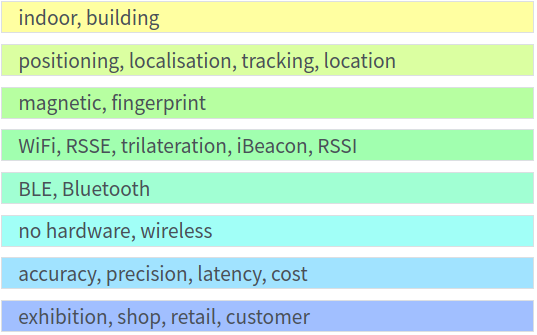
\includegraphics[width=0.48\textwidth]{img/patents/color.png}
    \caption{.}
    \label{fig:Patent-highlighting}
\end{figure}

Patents search highlighting categories which were used to build the classifier.

\begin{figure}[h]
    \centering
    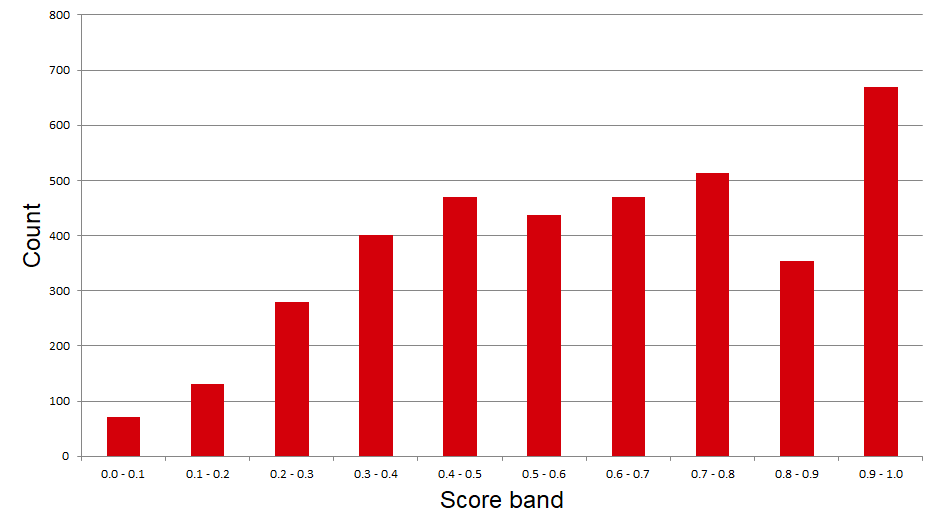
\includegraphics[width=0.48\textwidth]{img/patents/score.png}
    \caption{Patents result score of final report.}
    \label{fig:Patent-score}
\end{figure}

Result score shown on the \ref{fig:Patent-score} show how patents fit the classifier.


Second part is focused on building a model of a product and optimizing it for several criteria.
We focus on the system architecture of indoor positioning solutions. The system architecture provided by the Indoor Location Alliance is used as the main reference. Next we use the data from the Microsoft indoor positioning competition. This is a valuable data, because it provides data about development of indoor positioning technologies and their performance. Data of teams who are competing in the same conditions are perfect for benchmarking. Having the data of benchmarking, we may define technology complexity in real numbers and use it when builing the strategy.
% For this we use OPM (object process management) models and OPCAT simulator, UML diagrams, risk matrice and code based models containing figure of merits interconnections. We don't do optimization of a product here, just list possible options with [] curves.

Third we do a financial valuation. We collect all data about product, market, marketing channells and model of sales together.
Having existing business model which is outside of the scope of this paper, we may identify numbers of sales and revenues.
We use the costs and amount of investments we need to complete this project.
We tune the finantial model to obtain the positive NPV. To be coherent with the product figures of merits, we also adjust values of the model to receive a non-dominated product on the market.

Next we do value at risk analysis. With the value at risk gain curve, we check different financial models.
 % comparing to the Pareto frontier.

After all procedures we come up with bunch of strategies from where we can choose one. Again, we can't make decisions based on this models, but we can check strategies performance and for different technical decisions.

\subsection{Intellectual Property, Publications}



\section{Results}

\subsubsection{Figures of merit}

\begin{table*}[]
\caption{Technology FOM's}
\label{tab:techFOM}
\resizebox{\textwidth}{!}{%
\begin{tabular}{|l|l|l|}
\hline
cost hardware, software & USD & cost or hardware rent to provide coverage of needed area with normal operating accuracy \\ \hline
accuracy & m & accuracy of localization, difference between real position and measurements \\ \hline
cost & f(USD/sqm) & the cost itself cannot be directly compared because of different types of implementation. Instead, the overall cost presented in several roadmaps is shown. \\ \hline
range & m & Not important factor, complexity and scalability are affected by this factor. Not representative, because of different types of implementation. Excluded from FOM's \\ \hline
additional requirements & \begin{tabular}[c]{@{}l@{}}USD;\\ year\end{tabular} & If yes, product is not applicable until they are not solved. Not implemented into model, technologies with additional requirements are mot mapped. (Infrastructure Requirements, Impacts and Notes) \\ \hline
Scalability & low/med/high & range of scalability, important factor to consider in strategy choice \\ \hline
Complexity & low/med/high & range of complexity, important factor to consider in strategy choice \\ \hline
Robustness &  & additional information of what affect the performance of technology \\ \hline
\end{tabular}%
}
\end{table*}

Lower figures in table are affecting the technology choise, but cannot be added into model, so they are not considered as the figures of merit, but listed in table to explain the reason of excluding them.

\begin{table}[]
\caption{Product FOM's}
\label{tab:ProductFOM}
\begin{tabular}{lll}
accuracy & m & accuracy of localization, RMS error between real position and measurements \\
development time & month & time to develop the product based on technology with specified accuracy
\end{tabular}%
\end{table}

We focus on the figures of merit which are important for product development, and we use product FOM's mostly\ref{tab:ProductFOM}.

\begin{table*}[]
\caption{Performance of different technologies from the indoor positioning competition}
\label{tab:my-competition}
\resizebox{\textwidth}{!}{%
\begin{tabular}{|l|l|l|l|l|}
\hline
Team & Technical Approach & dev.time & RMS error & Team’s Affiliation \\ \hline
1 & 2.4GHz Phase Offset & 60 & 0.72 & Lambda:4 Entwicklungen \\ \hline
2 & WiFi+Modulated LEDs & 12 & 2.04 & MSR Asia \\ \hline
3 & 2.4GHz Time-of-Flight & 72 & 2.03 & Freie Univ. Berlin \\ \hline
4 & Ultrasonic Time-of-Flight &  & 2.09 & CMU \\ \hline
5 & IR/Radio Time-of-Flight & 18 & 2.35 & Rutgers \\ \hline
6 & 2.4GHz Time-of-Flight & 5 & 2.58 & Wroclaw Univ. of Tech. MT-Silesia Sp. \\ \hline
7 & WiFi+Bluetooth+IMU & 24 & 2.72 & NextoMe \\ \hline
8 & Modulated Magnetic Signals & 24 & 3.83 & Univ. of Oxford \\ \hline
9 & SDR Time-of-Flight & 4 & 3.87 & Humboldt Univ. of Berlin \\ \hline
10 & Modulated Magnetic Signals & 90 & 3.96 & DFKI \\ \hline
11 & 2.4GHz Phase Offset & 24 & 4.04 & Greina Technologies \\ \hline
12 & WiFi+Sound Time-of-Flight & 12 & 8.91 & Xian Jiaotong Univ. \\ \hline
13 & Steerable Antennas ToF & 12 & 10.22 & I.E.C.S. \\ \hline
14 & Bayesian Filter + WiFi Fingerprinting & 96 & 1.56 & Cork Institute of Technology \\ \hline
15 & WiFi+IMU Fingerprinting + Neural Network & 36 & 1.96 & Univ. of Cyprus/Cywee \\ \hline
16 & WiFi Fingerprinting + Neural Network & 12 & 2.22 & Nanyang Tech. Univ. \\ \hline
17 & WiFi+IMU Fingerprinting & 9 & 2.81 & Ubee S.A. \\ \hline
18 & WiFi+IMU Fingerprinting + Particle Filter & 24 & 3.19 & MSR Asia \\ \hline
19 & WiFi Time-of-Flight + Adaptive Filter & 12 & 3.47 & ETH/IMDEA/Armasuisse \\ \hline
20 & WiFi+IMU+Maps + Conditional Random Fields & 12 & 3.71 & Univ. of Oxford \\ \hline
21 & WiFi+Magnetic Fingerprinting + Particle Filter & 12 & 4.86 & Nanyang Tech. Univ. \\ \hline
22 & WiFi+IMU Fingerprinting + Clustering/Decision Trees & 3 & 5.23 & Tata Consulting Services \\ \hline
\end{tabular}%
}
\end{table*}

Technological limits

3 types: radio (distance), image (angle), fingerprinting (position).

Radio (multilateration, distance measurement), fingerprinting: noise level, wave reflections, sensor errors are main limitations.
Because of noise, the technology limit can’t be reached, only on frequencies where is no external noise, wave reflections - scanning error depends on geometry of signal way.
Image based: accuracy/precision of localisation depends on camera angle resolution. Because trilateration with camera is not possible, error is a linear function of range.



\subsection{State of the art}

\begin{table*}[h!]
\caption{technology comparison}
\label{tab:tech-comparison}
\resizebox{\textwidth}{!}{%
\begin{tabular}{|l|l|l|l|l|l|}
\hline
\textbf{IPS Technology}       & \textbf{Type}  & \textbf{Accuracy, m} & \textbf{Scalability} & \textbf{Complexity} & \textbf{Cost} \\ \hline
Geomagnetic                   & fingerprinting & 2                    & Low                  & Low                 & Very Low      \\ \hline
Photo                         & camera         & 1-10                 & Low                  & High                & High          \\ \hline
Barcodes                      & camera         & 1-10                 & Medium               & Low                 & Low           \\ \hline
Video, AR                     & camera         & 1-10                 & Low                  & High                & High          \\ \hline
Bluetooth Low Energy (BLE)    & Radio          & 1-3                  & High                 & Medium              & Medium        \\ \hline
RFID, Active                  & Radio          & 1-10                 & Medium               & Medium              & Medium        \\ \hline
RFID, Passive                 & Radio          & 1-10                 & Medium               & Medium              & Medium        \\ \hline
Wi-Fi                         & Radio          & 5-10                 & High                 & Medium              & Low           \\ \hline
Ultra Wide Band (UWB)         & Radio          & 0.15-0.5             & Low                  & Medium              & Medium to Low \\ \hline
Zigbee                        & Radio          & 3-5                  & Low                  & Low                 & Low           \\ \hline
FM                            &                & 2-4                  & Low                  & Low                 & Low           \\ \hline
Lighting-Based – Infrared LED & Lighting       & 0.15-3               & Low                  & Low                 & Low           \\ \hline
Lighting-Based – Visible LED  & Lighting       & 0.3-3                & Low                  & Low                 & Low           \\ \hline
Audible                       & sonic          & 0.5                  & Low                  & Low                 & Low           \\ \hline
Ultrasound                    & sonic          & 0.05-0.25            & Low                  & Medium              & Low to Medium \\ \hline
Inertial                      & supplementary  &                      & Low                  & Low                 &               \\ \hline
Pressure                      & supplementary  &                      &                      &                     &               \\ \hline
GPS                           & supplementary  & 6-10                 & Low                  & High                &               \\ \hline
\end{tabular}%
}
\end{table*}


\subsubsection{Positioning}
% companies positioning on market

We have to find products of this companies and other popular products to provide the landscape of market.


Number of patents is a valuable metric but it doesn't show us a value of patent, for example, Indooratlas OY obtain patents for magnetic fingerprinting technology which are more valuable now. Some huge companies such as Google LLC and Hitachi are not properly listed. They obtain higher number of patents that shown here, but all of them are not related to indoor navigation, so they are excluded from analysis. Excluding several companies is possible because best products are well known and we want to map products especially.

\cite{Security} It provides information about relative accuracy, mobile device battery usage and other system performance factors to help support early IPS planning and preliminary product evaluation.

\cite{Mautz2012IndoorPT}

IndoorAtlas research of 2016\cite{IPTrise} is a market landscape, which covers most popular technologies, market drivers and future trends. The paper covers adoption and drivers of indoor positioning systems, perspectives of geomagnetic indoor positioning.

Paper \cite{Brena2017} present a comparison of indoor positioning approaches.

% \cite{Kj_fingerprinting, Ashraf_deepnn, Li_geomagnetic, Mautz2012IndoorPT, 8859264, Infsoft_wp}

\begin{table}[]
\caption{Product index}
\label{tab:productstolink}
\begin{tabular}{|l|l|}
\hline
 & Products \\ \hline
P1 & Mapsted navigation deluxe \\ \hline
P2 & HERE Indoor Positioning (SDK \& radio mapper) \\ \hline
P3 & IndoorAtlas \\ \hline
P4 & VisioGlobe indoor navigation \\ \hline
P5 & Google VPS (visual positioning system) \\ \hline
\end{tabular}%
\end{table}

% Please add the following required packages to your document preamble:
% \usepackage{graphicx}
\begin{table}[]
\caption{Techologies index}
\label{tab:techindex}
\begin{tabular}{|l|l|}
\hline
index & sensors \\ \hline
T1 & GSM / 3G / 4G (LTE) \\ \hline
T2 & compass, magnetic fields \\ \hline
T3 & Wi-Fi \\ \hline
T4 & Bluetooth \\ \hline
T5 & accelerometer, gyroscope, pedometer \\ \hline
T6 & UWB antennas \\ \hline
T7 & Barometer \\ \hline
T8 & Camera \\ \hline
T9 & RFID, NFC, QR code \\ \hline
\end{tabular}%
\end{table}

We use the linking grid to map products \ref{tab:productstolink} to technologies \ref{tab:techindex}. To make table more compact, we use indexes.  

\begin{table*}[ht]
\caption{Technology comparison. Linking grid.}
\label{tab:linking_grid}
\resizebox{\textwidth}{!}{%
\begin{tabular}{lllllllllll|l|l|l|l|l|}
\cline{12-16}
 &  &  &  &  &  &  &  &  &  &  & \multicolumn{5}{l|}{Products} \\ \cline{12-16} 
 &  &  &  &  &  &  &  &  &  &  & \multicolumn{4}{l|}{current} & future \\ \cline{11-16} 
 &  &  &  &  &  &  &  &  & \multicolumn{1}{l|}{} & Markets & p1 & p2 & p3 & p4 & p5 \\ \cline{11-16} 
 &  &  &  &  &  &  &  & \multicolumn{2}{l}{} & positioning & x & x & x & x & x \\ \cline{11-16} 
 &  &  &  &  &  &  &  &  & \multicolumn{1}{l|}{} & marketing & x &  & x &  & x \\ \cline{11-16} 
 &  &  &  &  &  &  &  &  & \multicolumn{1}{l|}{} & analytics &  &  & x & x & x \\ \cline{11-16} 
 &  &  &  &  &  &  &  &  &  &  &  &  &  &  &  \\ \cline{2-16} 
\multicolumn{1}{l|}{} & \multicolumn{9}{l|}{Technologies} &  &  &  &  &  &  \\ \cline{2-16} 
\multicolumn{1}{l|}{} & \multicolumn{1}{l|}{T1} & \multicolumn{1}{l|}{T2} & \multicolumn{1}{l|}{T3} & \multicolumn{1}{l|}{T4} & \multicolumn{1}{l|}{T5} & \multicolumn{1}{l|}{T6} & \multicolumn{1}{l|}{T7} & \multicolumn{1}{l|}{T8} & \multicolumn{1}{l|}{T9} & Processes &  &  &  &  &  \\ \cline{2-16} 
\multicolumn{1}{l|}{} & \multicolumn{1}{l|}{x} & \multicolumn{1}{l|}{x} & \multicolumn{1}{l|}{x} & \multicolumn{1}{l|}{} & \multicolumn{1}{l|}{} & \multicolumn{1}{l|}{} & \multicolumn{1}{l|}{} & \multicolumn{1}{l|}{x} & \multicolumn{1}{l|}{x} & geofencing &  &  & x &  & x \\ \cline{2-16} 
\multicolumn{1}{l|}{} & \multicolumn{1}{l|}{} & \multicolumn{1}{l|}{} & \multicolumn{1}{l|}{x} & \multicolumn{1}{l|}{x} & \multicolumn{1}{l|}{} & \multicolumn{1}{l|}{x} & \multicolumn{1}{l|}{} & \multicolumn{1}{l|}{} & \multicolumn{1}{l|}{x} & asset tracking &  &  & x & x &  \\ \cline{2-16} 
\multicolumn{1}{l|}{} & \multicolumn{1}{l|}{x} & \multicolumn{1}{l|}{x} & \multicolumn{1}{l|}{x} & \multicolumn{1}{l|}{x} & \multicolumn{1}{l|}{x} & \multicolumn{1}{l|}{} & \multicolumn{1}{l|}{x} & \multicolumn{1}{l|}{x} & \multicolumn{1}{l|}{} & human real-time positioning & x & x & x & x & x \\ \cline{2-16} 
\multicolumn{1}{l|}{} & \multicolumn{1}{l|}{} & \multicolumn{1}{l|}{x} & \multicolumn{1}{l|}{x} & \multicolumn{1}{l|}{x} & \multicolumn{1}{l|}{} & \multicolumn{1}{l|}{} & \multicolumn{1}{l|}{} & \multicolumn{1}{l|}{} & \multicolumn{1}{l|}{} & queue management &  &  & x & x &  \\ \cline{2-16} 
\multicolumn{1}{l|}{} & \multicolumn{1}{l|}{} & \multicolumn{1}{l|}{} & \multicolumn{1}{l|}{x} & \multicolumn{1}{l|}{} & \multicolumn{1}{l|}{x} & \multicolumn{1}{l|}{x} & \multicolumn{1}{l|}{x} & \multicolumn{1}{l|}{} & \multicolumn{1}{l|}{x} & Sensor Fusion SLAM &  &  & x &  &  \\ \cline{2-16} 
\multicolumn{1}{l|}{} & \multicolumn{1}{l|}{x} & \multicolumn{1}{l|}{x} & \multicolumn{1}{l|}{x} & \multicolumn{1}{l|}{x} & \multicolumn{1}{l|}{x} & \multicolumn{1}{l|}{x} & \multicolumn{1}{l|}{x} & \multicolumn{1}{l|}{x} & \multicolumn{1}{l|}{} & map creation & x & x & x & x & x \\ \cline{2-16} 
\multicolumn{1}{l|}{} & \multicolumn{1}{l|}{} & \multicolumn{1}{l|}{} & \multicolumn{1}{l|}{} & \multicolumn{1}{l|}{} & \multicolumn{1}{l|}{} & \multicolumn{1}{l|}{} & \multicolumn{1}{l|}{} & \multicolumn{1}{l|}{} & \multicolumn{1}{l|}{} & Product phase &  &  &  &  &  \\ \hline
\multicolumn{1}{|l|}{mature} & \multicolumn{1}{l|}{} & \multicolumn{1}{l|}{} & \multicolumn{1}{l|}{} & \multicolumn{1}{l|}{x} & \multicolumn{1}{l|}{} & \multicolumn{1}{l|}{} & \multicolumn{1}{l|}{} & \multicolumn{1}{l|}{} & \multicolumn{1}{l|}{} & Research &  &  & x & x & x \\ \hline
\multicolumn{1}{|l|}{growth} & \multicolumn{1}{l|}{} & \multicolumn{1}{l|}{} & \multicolumn{1}{l|}{x} & \multicolumn{1}{l|}{} & \multicolumn{1}{l|}{x} & \multicolumn{1}{l|}{x} & \multicolumn{1}{l|}{} & \multicolumn{1}{l|}{x} & \multicolumn{1}{l|}{} & Development & x & x & x & x & x \\ \hline
\multicolumn{1}{|l|}{emerging} & \multicolumn{1}{l|}{} & \multicolumn{1}{l|}{x} & \multicolumn{1}{l|}{} & \multicolumn{1}{l|}{} & \multicolumn{1}{l|}{} & \multicolumn{1}{l|}{} & \multicolumn{1}{l|}{} & \multicolumn{1}{l|}{} & \multicolumn{1}{l|}{} & Delivery &  &  & x & x &  \\ \hline
\multicolumn{1}{|l|}{declining} & \multicolumn{1}{l|}{x} & \multicolumn{1}{l|}{} & \multicolumn{1}{l|}{} & \multicolumn{1}{l|}{} & \multicolumn{1}{l|}{} & \multicolumn{1}{l|}{} & \multicolumn{1}{l|}{x} & \multicolumn{1}{l|}{} & \multicolumn{1}{l|}{x} & Support & x & x & x & x &  \\ \hline
\end{tabular}%
}
\end{table*}

In linking grid \ref{tab:linking_grid}, we map technologies to possible processes in indoor positioning systems. For each technology, we identify the technology adoption or readiness level in simplest form. After that, for each process, we mark all possible technologies involved. Then we mark products to markets and identify which processes are involved into each product, on which markets the product is positioned and what the level of this product on the market. 


\subsubsection{Patents}

\begin{figure}[h]
    \centering
    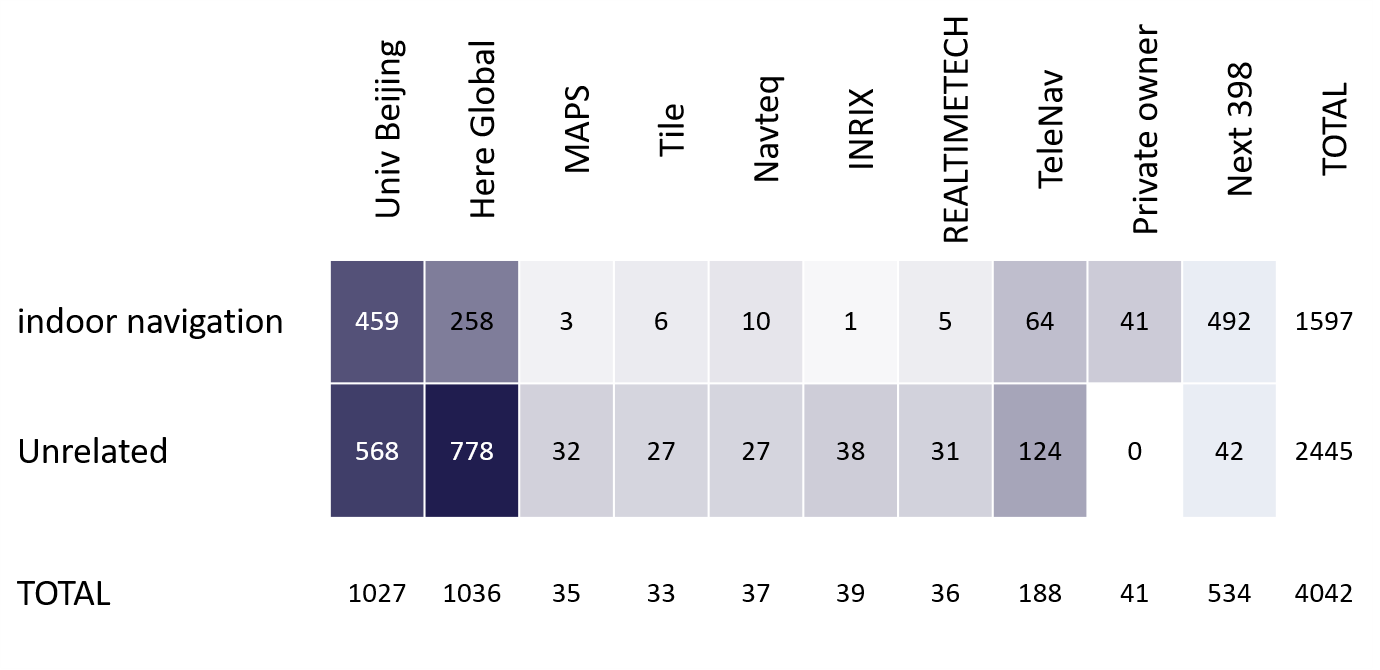
\includegraphics[width=0.48\textwidth]{img/patents/Patenting2.png}
    \caption{Portfolio size: Active patent families, by organisation and technology. Currently active patent families (granted or pending) by organisation and technology.}
    \label{fig:Patent-families2}
\end{figure}

In patent research of current field, we use patent classifier with the training set of 590 positive and 136 negative patents marked.
Using this classifier and AI patent platform cipher.ai, we do the organisation search which is presented on \ref{fig:Patent-families2}
. On the Figure \ref{fig:Patent-families2} category of "Unrelated" is the category of patents that does not fit the classifier.

\begin{figure}[h]
    \centering
    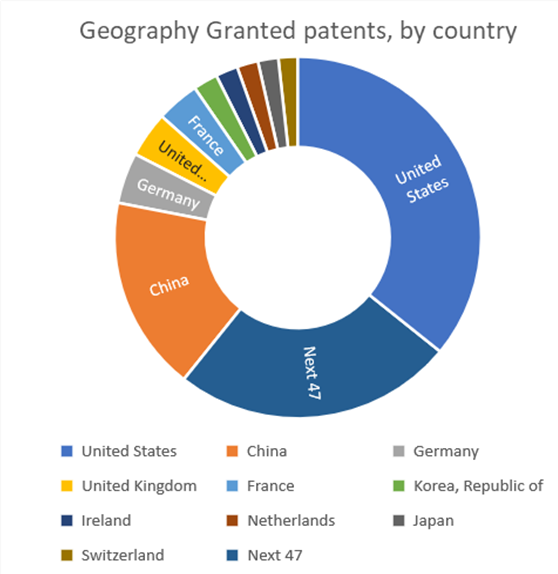
\includegraphics[width=0.48\textwidth]{img/patents/Granted patents by country and organisation.png}
    \caption{}
    \label{fig:Patent-u}
\end{figure}



\begin{figure*}[h]
    \centering
    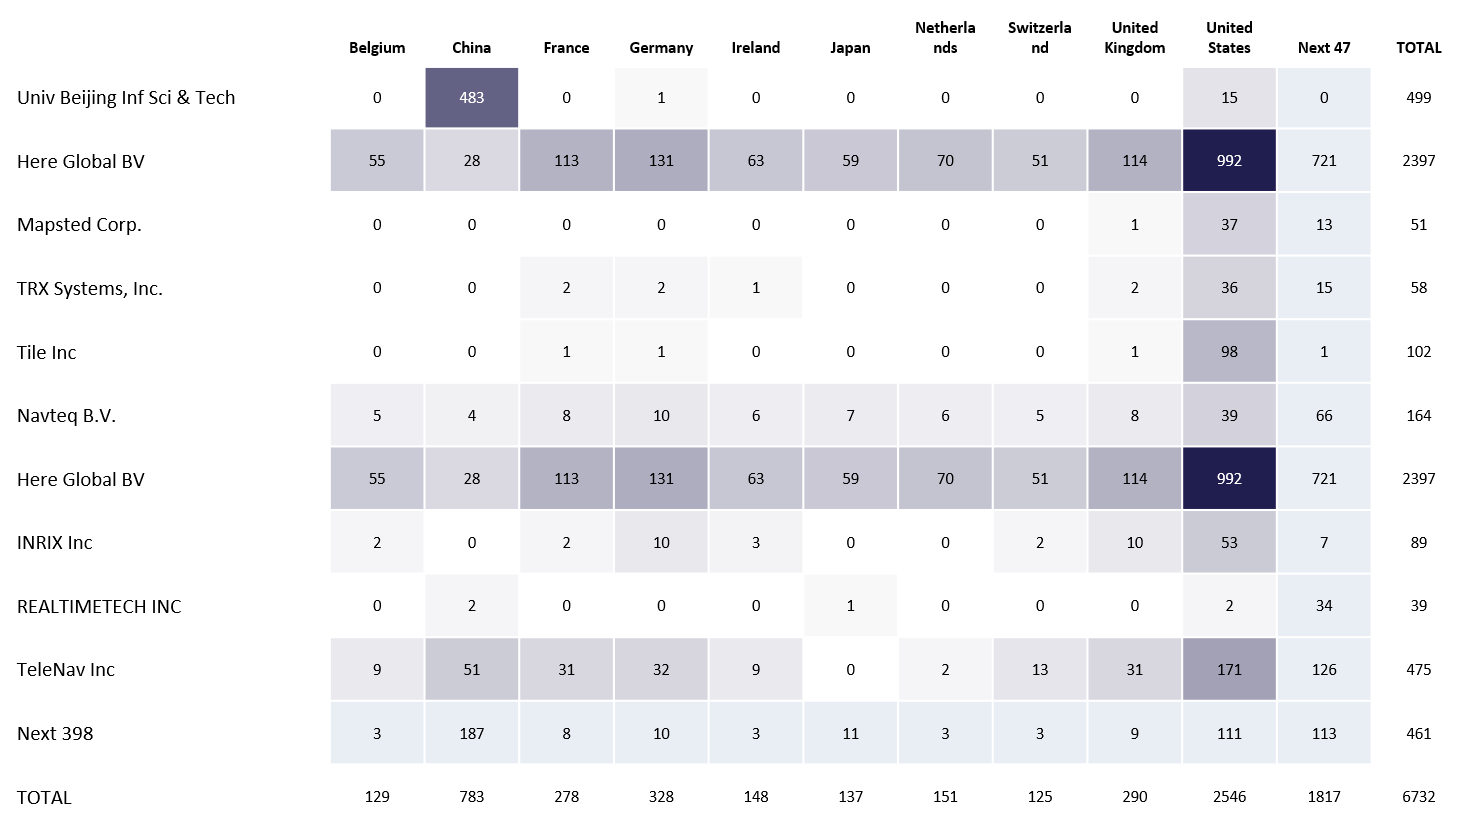
\includegraphics[width=\textwidth]{img/patents/Geography Granted patents by country and organisation.png}
    \caption{Geography: Granted patents, by country and organisation
Currently active and granted individual patents per country, by organisation.}
    \label{fig:Granted-patents-by-coutry}
\end{figure*}



\begin{table*}[]
\caption{Portfolio size: Active patent families, by organization and technology}
\label{tab:patents-scope}
\resizebox{\textwidth}{!}{%
\begin{tabular}{lllllllllll}
 & Univ Beijing & Here Global & MAPS & Tile & Navteq & REALTIMETECH & TeleNav & Private owner & Next 398 & TOTAL \\
indoor navigation & 459 & 258 & 3 & 6 & 10 & 5 & 64 & 41 & 492 & 1597 \\
Unrelated & 568 & 778 & 32 & 27 & 27 & 31 & 124 & 0 & 42 & 2445 \\
TOTAL & 1027 & 1036 & 35 & 33 & 37 & 36 & 188 & 41 & 534 & 4042
\end{tabular}%
}
\end{table*}


\begin{table*}[]
\caption{Geography: Granted patents, by country and organization}
\label{tab:patents-map}
\resizebox{\textwidth}{!}{%
\begin{tabular}{lllllllllllll}
 & Belgium & China & France & Germany & Ireland & Japan & Netherlands & Switzerland & United Kingdom & United States & Next 47 & TOTAL \\
Univ Beijing Inf Sci \& Tech & 0 & 483 & 0 & 1 & 0 & 0 & 0 & 0 & 0 & 15 & 0 & 499 \\
Here Global BV & 55 & 28 & 113 & 131 & 63 & 59 & 70 & 51 & 114 & 992 & 721 & 2397 \\
Mapsted Corp. & 0 & 0 & 0 & 0 & 0 & 0 & 0 & 0 & 1 & 37 & 13 & 51 \\
TRX Systems, Inc. & 0 & 0 & 2 & 2 & 1 & 0 & 0 & 0 & 2 & 36 & 15 & 58 \\
Tile Inc & 0 & 0 & 1 & 1 & 0 & 0 & 0 & 0 & 1 & 98 & 1 & 102 \\
Navteq B.V. & 5 & 4 & 8 & 10 & 6 & 7 & 6 & 5 & 8 & 39 & 66 & 164 \\
Here Global BV & 55 & 28 & 113 & 131 & 63 & 59 & 70 & 51 & 114 & 992 & 721 & 2397 \\
INRIX Inc & 2 & 0 & 2 & 10 & 3 & 0 & 0 & 2 & 10 & 53 & 7 & 89 \\
REALTIMETECH INC & 0 & 2 & 0 & 0 & 0 & 1 & 0 & 0 & 0 & 2 & 34 & 39 \\
TeleNav Inc & 9 & 51 & 31 & 32 & 9 & 0 & 2 & 13 & 31 & 171 & 126 & 475 \\
Next 398 & 3 & 187 & 8 & 10 & 3 & 11 & 3 & 3 & 9 & 111 & 113 & 461 \\
TOTAL & 129 & 783 & 278 & 328 & 148 & 137 & 151 & 125 & 290 & 2546 & 1817 & 6732
\end{tabular}%
}
\end{table*}


\subsection{Building a model}

% What points are we roadmap?

% usage of technology
% possible applications



\subsubsection{Architecture}

One way of AI usage with indoor positioning system is shown in post of IBM-research group \cite{AI-Centric_IPS}. This gives us some view of achitecture and data transactions in modern IPS applications.

\begin{figure}[h]
    \centering
    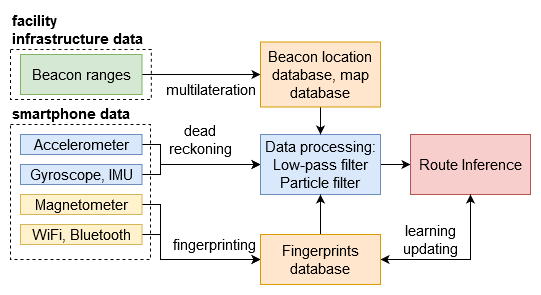
\includegraphics[width=0.48\textwidth]{img/indoor navigation roadmap-Page-3.png}
    \caption{Signal processing system architecture}
    \label{fig:arch}
\end{figure}

On figure \ref{fig:arch} we present possible architecture of indoor positioning application.
We use blue color for dead-reckoning application. Because of different smartphone sensors, signal processing will be different for every smartphone model, that's why signal processing should be done on the smartphone itself.

After first signal filtering from inertial and others complementary sensors (barometer), all information from sensors has to be matched with fingerprint database and map databases. This process can be done on the remote server or locally, this depends on system architecture chosen.

The technology choice of system architecture can't be explained, because there is no single strategy for system design.

Only several assumptions can be presented:

\begin{itemize}[noitemsep]
\item Server based systems can be provided by an external vendor - buying a service
\item Server based systems are enough cost effective to be used (development of server platforms in 2020 is enough to not care about signal processing on the local devices)
\item Mobile device based are harder in development and support
\item Mobile device based systems may not require external server and can be run locally - stable work with no internet connection
\item Once operating, mobile device based are cheaper, because no server support and rent needed - costs are on user side. Important for scalability (if one million of users will use system, some additional traffic management will be required)
\item Emergency help services shall not depend on internet connection - broadcast systems, mobile device used as transmitter - mobile device initiated systems
\item In some cases network initiated positioning can be useful. For example, if ultrasound waves are used for positioning, sound transmission will happen over short periods of time defined by network, this will reduce level of noise.
\end{itemize}

For the most common case of human tracking with no special requirements on internet connection, scalability and sensors used, architecture shown of \ref{fig:arch} can be used.

\begin{figure}[h]
    \centering
    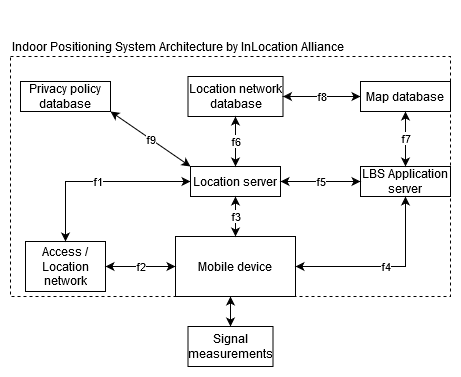
\includegraphics[width=0.48\textwidth]{img/InLocation Alliance (ILA).png}
    \caption{InLocation Alliance (ILA) system architecture}
    \label{fig:arch2}
\end{figure}

InLocation Alliance (ILA) was founded in 2012 and worked on indoor positioning solutions. In 2014 the ILA created an open, technology-independent architecture in support of accurate location of mobile devices within different types of indoor venues (see Figure \ref{fig:arch2}), which presents seven key system elements and nine interfaces.

What we see from Figure \ref{fig:arch2}, is that only mobile devices are considered as input, current architecture don't have beacons in it.

Results of ILA work and standards they make are not open and published, so they are not a standard now and we may freely update this structure.
Moreover, in \cite{Security} author propose to define both system architecture diagrams \ref{fig:arch} and \ref{fig:arch2} and use them as a product documentation to describe interfaces and so on.

% The ILA System Architecture (SA) specifies the main components and interface requirements of a technology-independent system architecture for indoor location.

% The SA has been designed to support a wide range of venues: from the very small (e.g. stand-alone business) to the very large (e.g. corporate campus) to the very distributed (e.g. worldwide retail chain).
% The SA is based on open interfaces in order to support multi-vendor environments for indoor location.
% While the SA in itself is generic and technology agnostic, the focus of the first public release of the SA is on Wi-Fi and BT.

\subsubsection{Roadmap system modelling}
% \subsubsection{Roadmap model in OPM}

From \cite{Security}, the process of documenting architecture can be described as:

At the appropriate times, take steps with prospective system providers:
\begin{itemize}[noitemsep]
\item Provide the two architecture diagrams to prospective vendors
\item Ask vendors to document the architecture and positioning mode(s) of the IPS being considered, relative to these architecture diagrams.
\item Plan and document any data import or export functions.
\item Review the existing system’s reporting capabilities against \ what reporting requirements apply for business uses of the system.
\item Review what applications reside where, such as an on-premises server or a cloud server.
\end{itemize}

We will create an OPM model using this approach and Figures \ref{fig:arch} and \ref{fig:arch2}.

\begin{figure*}[h]
    \centering
    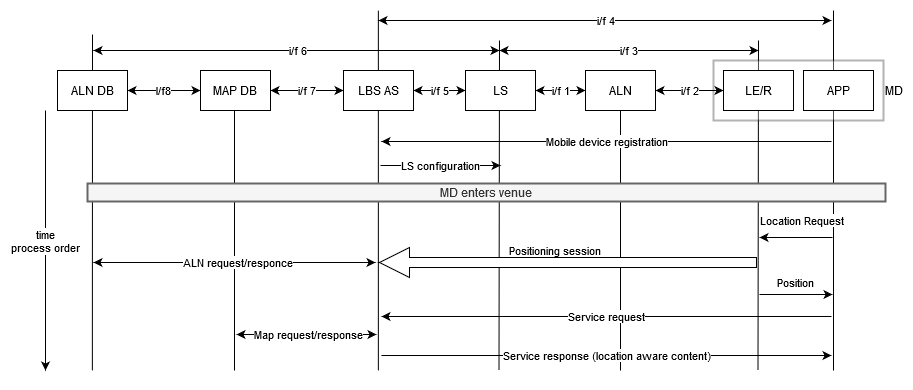
\includegraphics[width=\textwidth]{img/location aware content by ILA.png}
    \caption{Location aware content example by ILA.}
    \label{fig:loc_aware}
\end{figure*}

We present an example from \cite{ILA-System-Architecture} of how location aware content is delivered to users.
On Figure \ref{fig:loc_aware}, we see the order of steps, used to provide location aware content to user, e.g. geo-targeting or geo-fencing. This diagram doesn't explain much the structure and interfaces of system architecture, but shows some connections between them. All short naming are the same as in Figure \ref{fig:arch2}.

% For better structure representation we will use OPM models.



\subsection{Technology Strategy Vision}

% explain vision and strategy

From annual reports\cite{trends2017,trends2019} we can get history of trends in mobile marketing. When and where it is possible,different technologies and services are implemented in IPS. We will list several trends of indoor positioning systems.


Merge of indoor and outdoor positioning systems:
It is visible that IPS technologies are converging to some set of technologies. When this will happen, the connection between IPS and GPS or other outdoor positioning systems can be done. Right now, several IPS products support this feature, but this is not a global solution.\cite{Brena2017}
Privacy and security in IPS development:
Current trends with protection of users in web (GDPR policies) bring us to the point that some steps in this direction are done by government. Development of a product which is privacy safe can improve the adoption of use, which is important factor now. This factor directly affects the scalability of specific technologies and products.\cite{Brena2017}
Crowd-source mapping:
Most of technologies used in IPS systems requires hours of measurements inside the facilities to create a map of a building. Regular users can provide big amount of measurements, needed to create map of building and update it regularly.  This approach is important for applications that don't require special equipment for measurements and need regular map update (magnetic fields, WiFi, ambient sound localization technologies).\cite{Brena2017}
"China Crisis Ebbs, But Tracking Apps Are Going Strong" - the article of today's paper in The New York Times \cite{Tracking_Apps_times}.
Having the great need of tracking people, new products of human tracking were developed rapidly. "But the authorities have set few limits on how that data can be used. And now,officials in some places are loading their apps with new features, hoping the software will live on as more than just an emergency measure."
Indoor Location of E911 Mobile Callers:
Enhanced 911 Services enable 911 operators to:
Immediately pinpoint the location of the 911 caller based on the calling number
Callback the 911 caller if a disconnect occurs
Tracking location of people in emergency situation is an important challenge and one of the most important drivers of current IPS technology.
The initiative shown some results in 2013, but USA government requires universal service that will be implemented across the USA. One of the key points of this measure, that it has to work indoors. Importance of E911 point is that several actions are already done and several technological steps may change the state of USA market which may happen in future 2-5 years.

The overall strategy is to deliver the product in least development time, while reaching the average accuracy.

\subsection{Timeline}

We use data of Microsoft competition as a starting reference. In table \ref{tab:my-competition}, we have time of development and resulting accuracy for the different technology choice of different teams participated.
We may use these dependencies to understand, what time is needed to achieve each level of accuracy for different combinations of technologies.

\begin{figure}
  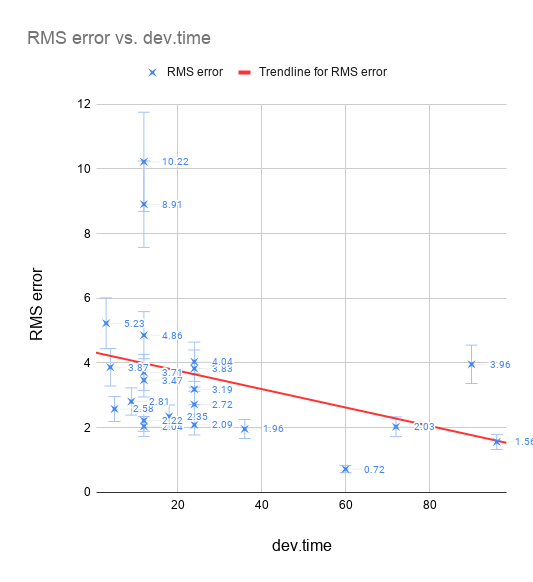
\includegraphics[width=0.49\textwidth]{img/RMSerrorvsdevtime.png}
  \caption{Root mean square error of positioning versus time of development}
  \label{im:rmse}
\end{figure}

On figure \ref{im:rmse}, we see the team competitors performance versus time for development in months.

\begin{table}[]
\caption{Technology choice.}
\label{tab:best-tech}
\begin{tabular}{lll}
Technical Approach & dev.time & RMS error \\
SDR Time-of-Flight & 4 & 3.87 \\
2.4GHz Time-of-Flight & 5 & 2.58 \\
WiFi+IMU Fingerprinting & 9 & 2.81 \\
WiFi+Modulated LEDs & 12 & 2.04 \\
WiFi Fingerprinting + Neural Network & 12 & 2.22 \\
WiFi+IMU Fingerprinting + Neural Network & 36 & 1.96 \\
2.4GHz Phase Offset & 60 & 0.72 \\
Bayesian Filter + WiFi Fingerprinting & 96 & 1.56
\end{tabular}%
\end{table}

We choose the best performance in technologies \ref{tab:best-tech} by multiplication of all of parameters.
Performance = 1 / (development time * accuracy).

We predict the accuracy of or product in between of optimal scenario (non-dominated points) and the trend line. From this we may present a timeline.

\begin{figure*}[t]
    \centering
    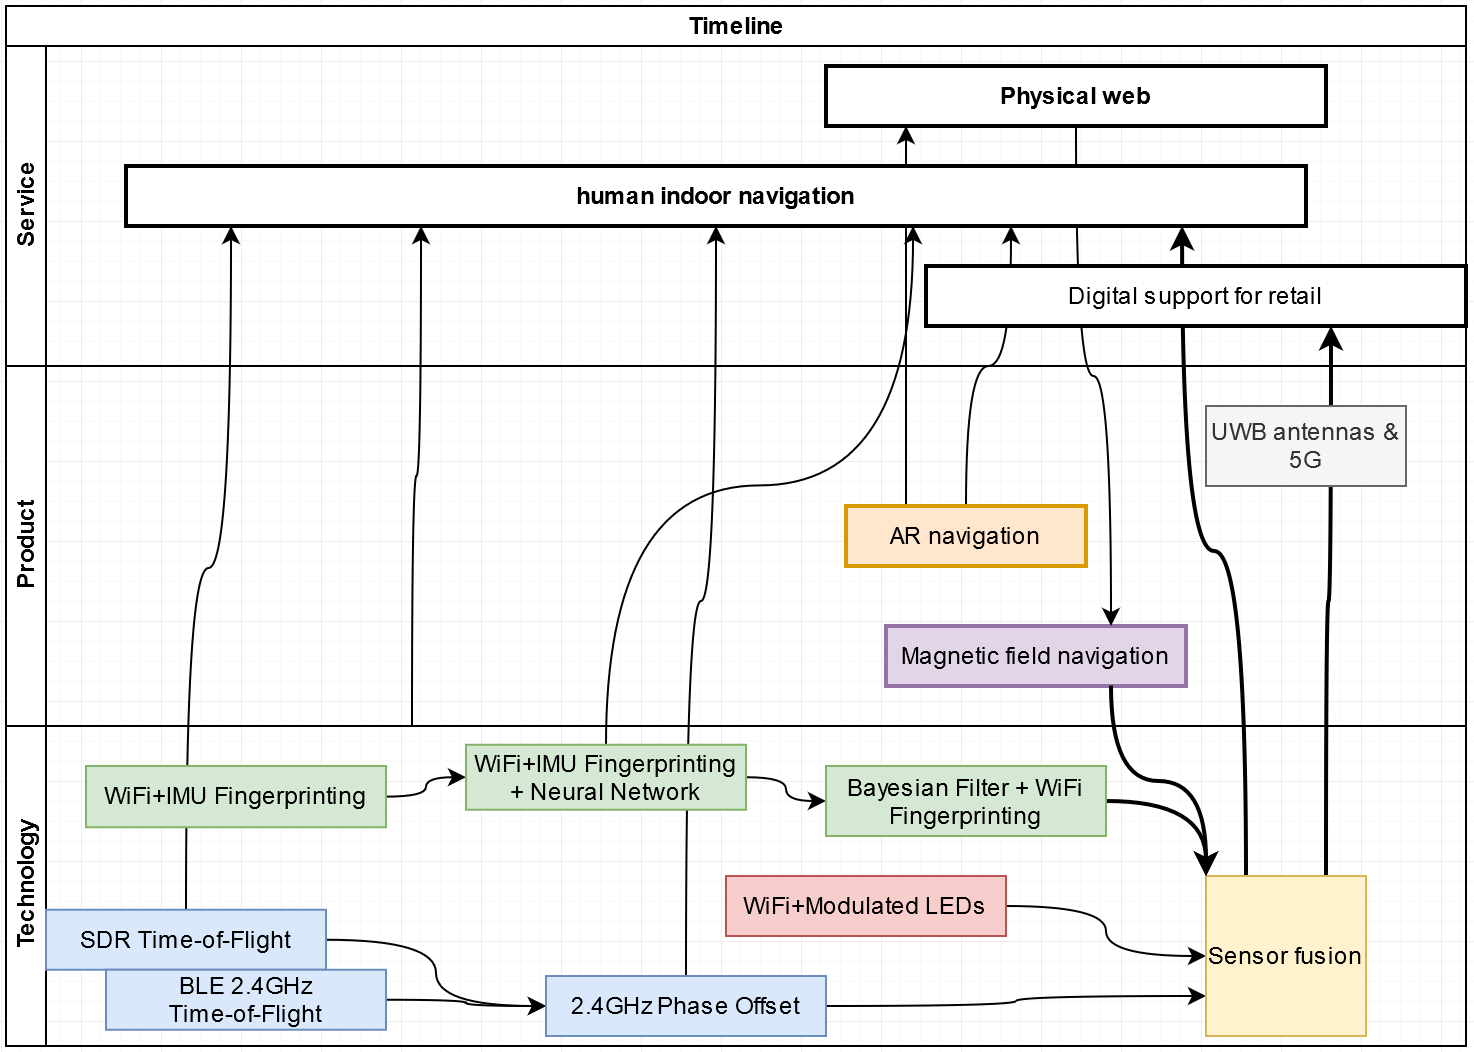
\includegraphics[width=0.9\textwidth]{img/timeline.png}
    \caption{Timeline diagram. Left to right: Passed term, Short term (1-2 years), Long term (2-5 years).}
    \label{fig:timeline}
\end{figure*}

On \ref{fig:timeline} we show the action plan for development the product with different alternative strategies.
 % historical evolution of trends in mobile technologies and technologies of indoor positioning.

The overall trend is that IPS products are converging to a global ecosystem - digitisation of cities. After human and assets will be tracked constantly, this will be a big supplementation to a smart cities technologies.
Before that, there is the market of IPS in retail applications (asset tracking, geo-fencing, way finding, proximity marketing).\cite{Infsoft_wp}

By speaking of current situation on the market, we can say that human indoor tracking is growing, but it is not mature.
We are building product with the main function of human indoor positioning as shown on Figure\ref{fig:timeline}.

Magnetic field navigation is another perspective factor in the timeline, some progress is already achieved by IndoorAtlas company in this field, but this technology will might become global and will assist the usual dead reckoning and existing WiFi and BLE technologies.

UWB localisation can be better than existing radio-based technologies, but until there is no UWB communication equipment in smartphones and facilities worldwide. Spreading of 5G may change this situation.
%
% The matchmaking apps are stated in the timeline, because it is the interest of current paper product research. This is the way of usage the IPS technology which merges social networks and geo-based services.
% \begin{wrapfigure}{l}{0.7\linewidth}
% 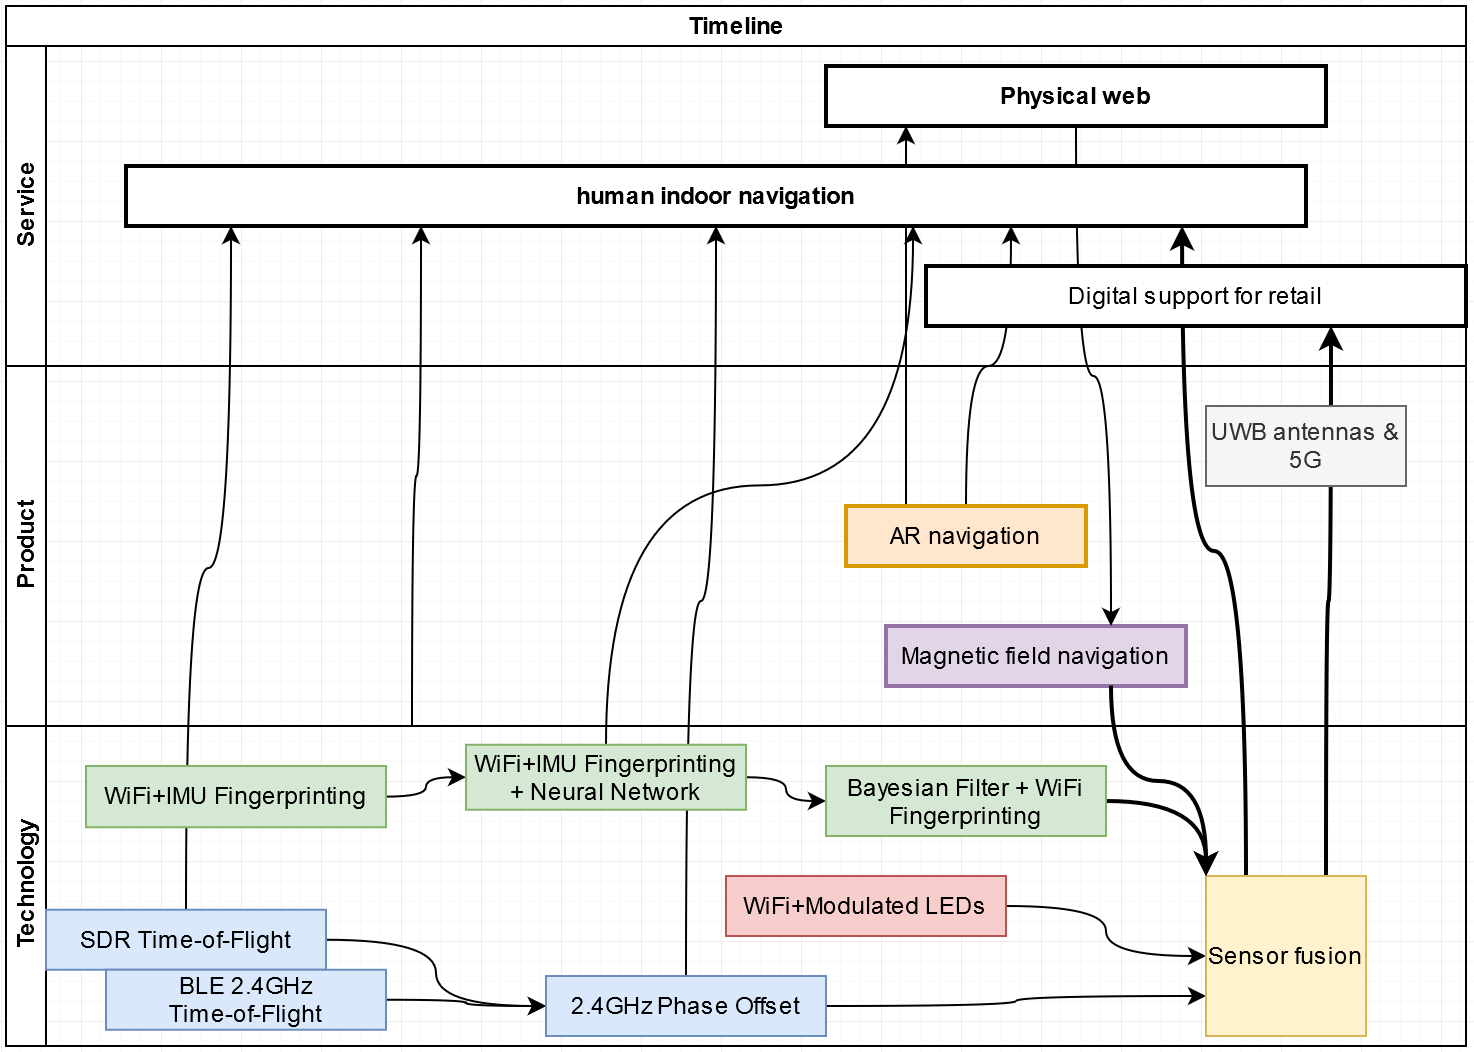
\includegraphics[width=\linewidth]{img/timeline.png}
% \caption{This is the former Share\LaTeX{} logo}
% \end{wrapfigure}
% To present current landscape, we will state known trends of this field.
% Because of uncertainty behind this information, in timeline they all can be marked under "Future applications".

\subsection{Technical feasibility}

Physical limits of indoor positioning system come from the environment. Real usage limits are more flexible and are directed by human limits (reaction time).

Applicable limits of each of FOM-s are different for different applications. For people to navigate, the accuracy of (1 m) and response frequency of (5 s)  may be enough. In big environment, the accuracy of 1-3 meters (similar to GPS performance) is enough. For the high performance applications, the accuracy must be lower than 1m (0.1 -0.5)m and response frequency near (0.1-0.5)s. In ARkit research[1] proposed model, where accuracy required is equal to 10 percent of the distance between various points of the destination, which gives us same 0.4-0.5m for rooms and 4-5m for big halls.


The range for RSSI method is calculated by formula:

$\mathbf{ dist = 10 * ((RSSI_{1m} - RSSI_{rec})/(10 * Path loss)) }$

Main limitation with this type of distance calculation is sensor's sensitivity and field noise. Having -96 DBm sensitivity and 4 DBm transmit power, system will be operable in range of 30m.

\begin{figure}
  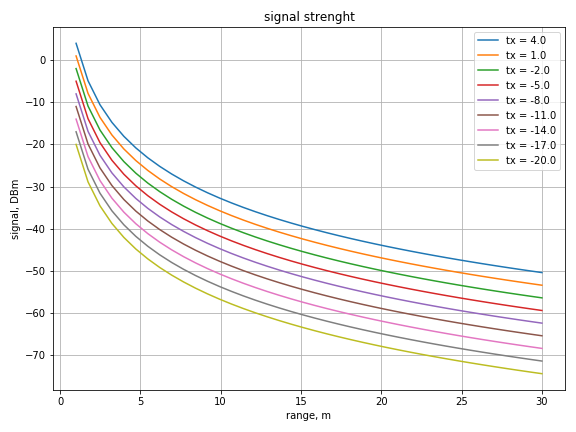
\includegraphics[width=0.49\textwidth]{img/signal_strenght.png}
  \caption{Radio signal strength distribution model.}
  \label{fig:signal}
\end{figure}
To calculate the signal distribution, we use Free-space path loss formula and Log-distance path loss model.

We use constants from signal measurements in [21], and Log-distance path loss model.

This gives us the information that signal transmission quality depends of distance, transmitter power and receiver sensitivity.

For BLE, we the normal conditions are as in figure above: with normal operating range of 30m, transmitter power in [4 DBm, -20 DBm] range, receiver sensitivity in range of -40 DBm, -60 DBm.

The limits for tracking technologies are not strict, they are only affecting accuracy and precision of localization. We can use table of normal ranges for technologies as a reference, but the performance will depend of huge amount of factors which can't be modeled accurately.

\subsection{Financial Valuation}

Customer Acquisition Cost (CAC)= (product cost+sales+marketing)÷(number of customers)

Life-Time Value (LTV) = (average value of sales) × (number of repeat transactions) × (average retention time)

Profit= LTV×(average margin)

Assumptions: 

\begin{enumerate}
    \item     an exhibition area of 1000 sqm, needs 9 BLE anchors for full coverage
    \item     Calculations for 1 day
    \item     1000 visitors per day
    \item     Mobile app development needs 4hrs of programming
    \item     1 person for hardware installation and removal
\end{enumerate}

Assumptions on revenues rate are shown on the figure above.

Plan A:

CAC~a~ to charge each booth (participating company) to benefit from indoor navigation facilities per day

Daily costs of operation = 1200 USD; Fixed costs = 3000 USD;

Plan B:

CAC~B~to charge each booth (participating company) to benefit from indoor navigation facilities + additional product features

Daily costs of operation = 1700 USD; Fixed costs = 2000 USD;

% \begin{figure}
%   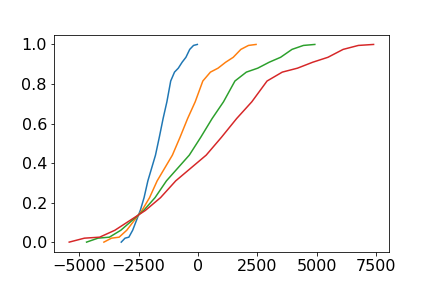
\includegraphics[width=0.49\textwidth]{img/fin/plan a.png}
%   \caption{Radio signal strength distribution model.}
%   \label{fig:signal}
% \end{figure}

\begin{figure}
  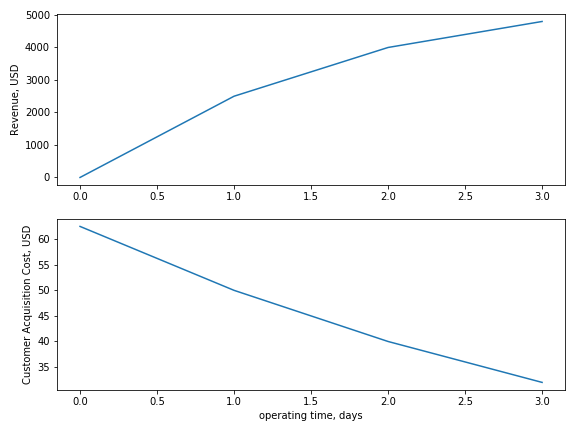
\includegraphics[width=0.49\textwidth]{img/fin/varg_10runs.png}
  \caption{Customer acquisition cost}
  \label{fig:cac}
\end{figure}

We assume that in strategies, CAC is different, and costs are different. Number of customers is assumed probabilistic as a triangular distribution. We use the assumption in the model, that for the longer operation time, customers get a discount as a power function of power 0.8.

The total revenue and customer acquisition cost are presented on the Figure \ref{fig:cac}. This is an example for one strategy, average customer acquisition is about 45 USD per day. Average revenue is about 1800 USD per day.

%We are modelling two strategies for operating time of 2 and 5 days.
%Watching on the figure, we understand that strategy A is better on a short term, and on a long operating time, both strategies are almost equal.


\begin{figure}
  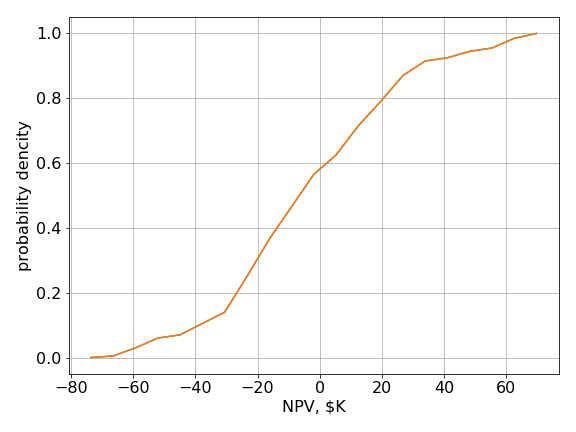
\includegraphics[width=0.49\textwidth]{img/fin/varg_mruns.png}
  \caption{Value at risk gain curve}
  \label{fig:signal}
\end{figure}

\section{Validation}


The tech background is validated by comparison of scientific publications \cite{ILA-System-Architecture}, \cite{Brena2017, Kj_fingerprinting, Li_geomagnetic, Mautz2012IndoorPT, AI-Centric_IPS} and analysis of the existing solutions.
The business model was sequentially developed to satisfy four fits model.
Expert validation (IndoorAtlas expert interview, customer interview).

One of the most valuable tools for the roadmap developing was benchmarking with existing researches \cite{microsoft}.


\section{Conclusions}
% 5. Conclusions & Lessons Learnt from TPR:F/TPR:A (10%)

The indoor navigation product strategy tool is in development now.
It was proven to be viable by customer discovery process and by revenue model & calculation.

However, in order use this tool efficiently, this strategy tool requires:
\begin{enumerate}
    \item to be accurate - proved to be possible but requires lot of engineering
    \item to be convenient - depends on the way of realization and would require continuous improvements
    \item the acceptance of the market segment, which shall be accurately chosen 
    \item complexity of either software or hardware
\end{enumerate}

This paper shows the usage of different modelling approaches, which allows to develop the strategy based on the product model.

Paper provides a roadmap, technology landscape and technology strategy choice that is based on the timeline and all relevant roadmap elements. 
Each statement is supported by a quantitative fact or analytics defined by the models of product and technology.

System model, created in this paper, list all important figures, components and capabilities. The key functions and system architecture are identified using common standards. Figures of merit identify capabilities and limits of technology and provide information about product development strategy. The demonstrators, patents, known products and products which can be used as a components of indoor positioning system are listed in paper and implemented into strategy.

In paper, we identify the limit for the product development performance as an average performance (root mean square trend line). This allow us to make a strategy choice, to develop a product/technology or to buy it. 

The financial valuation was developed, based on product model and sales models.
We use probabilistic models to develop strategy under uncertainty. Different scenarios (pessimistic, baseline, optimistic) are defined. 

% \section{References}


% \cite{Kj_fingerprinting, Ashraf_deepnn, Li_geomagnetic, Mautz2012IndoorPT}
% \cite{BLE_loc, microsoft}

\bibliographystyle{ieeetr}
% \bibliographystyle{unsrt}
\bibliography{literature}



\end{document}
